\documentclass[DaoFP]{subfiles}
\begin{document}
    \setcounter{chapter}{8}

    \chapter{自然变换 (Natural Transformations)}

    我们已经看到,当两个对象$a$和$b$是同构的时,它们会在箭头集之间生成双射(bijections),我们现在可以将其表达为态射集(hom-sets)之间的同构(isomorphisms)。对于所有$x$,我们有:
    \begin{align*}
        \mathcal{C}(a, x) &\cong \mathcal{C}(b, x) \\
        \mathcal{C}(x, a) &\cong \mathcal{C}(x, b)
    \end{align*}
    但反过来并不成立。态射集之间的同构并不会导致对象之间的同构,除非满足附加的自然性条件(naturality conditions)。我们现在将在逐步更一般的设置中重新表述这些自然性条件。

    \section{态射函子之间的自然变换 (Natural Transformations Between Hom-Functors)}

    一种可以建立两个对象之间同构的方法是直接提供两个箭头,一个是另一个的逆。但通常情况下,更容易间接地完成,通过定义箭头之间的双射,无论是作用在两个对象上的箭头,还是从两个对象发出的箭头。

    例如,正如我们之前所看到的,对于每一个$x$,我们可能有一个可逆的箭头映射$\alpha_x$。
    \[
        \begin{tikzcd}
            \node(x) at (0, 2) {x};
            \node(a) at (-2, 0) {a};
            \node(b) at (2, 0) {b};
            \node(c1) at (-1, 1.5) {};
            \node(c2) at (-1.5, 1) {};
            \node(c3) at (-1, 2) {};
            \node(c4) at (-2, 1) {};
            \node(d1) at (1, 1.5) {};
            \node(d2) at (1.5, 1) {};
            \node(d3) at (1, 2) {};
            \node(d4) at (2, 1) {};
            \node (aa) at (-1, 0.75) {};
            \node (bb) at (1, 0.75) {};
            \draw[->] (x) .. controls (c1)  and (c2) .. (a); % bend
            \draw[->, green] (x) .. controls (c3)  and (c4) .. (a); % bend
            \draw[->, blue] (x) -- (a);
            \draw[->] (x) .. controls (d1)  and (d2) .. (b); % bend
            \draw[->, green] (x) .. controls (d3)  and (d4) .. (b); % bend
            \draw[->, blue] (x) -- (b);
            \draw[->, red, dashed] (aa) -- node[above]{\alpha_x} (bb);
        \end{tikzcd}
    \]
    换句话说,对于每一个$x$,存在一个态射集的映射:
    \[ \alpha_x \colon \mathcal{C}(x, a) \to \mathcal{C}(x, b) \]

    当我们变化$x$时,这两个态射集成为两个反变函子(contravariant functors),$\cat C(-, a)$和$\cat C(-, b)$,$\alpha$可以看作它们之间的一个映射。这样的函子映射,称为变换(transformation),实际上是一个个别映射$\alpha_x$的集合,每个$\mathcal{C}$中的对象$x$都有一个映射。

    函子$\mathcal{C}(-, a)$描述了世界如何看待$a$,而函子$\mathcal{C}(-, b)$描述了世界如何看待$b$。

    变换$\alpha$在这两个视角之间来回切换。$\alpha$的每个分量$\alpha_x$表明,从$x$看$a$的视角与从$x$看$b$的视角是同构的。

    我们之前讨论过的自然性条件(naturality condition)是:

    \[ \alpha_y \circ (- \circ g) = (- \circ g) \circ \alpha_x \]
    它将取自不同对象的$\alpha$的分量联系起来。换句话说,它将由箭头$g \colon y \to x$连接的两个观察者$x$和$y$的视角联系起来。

    这个方程的两边作用在态射集$\mathcal{C}(x, a)$上。结果位于态射集$\mathcal{C}(y, b)$中。我们可以将两边重写为:
    \begin{align*}
        \cat C(x, a) \xrightarrow{(- \circ g)} \cat C(y, a) \xrightarrow{\alpha_y} \cat C(y, b) \\
        \cat C(x, a) \xrightarrow{\alpha_x}  \cat C(x, b)  \xrightarrow{(- \circ g)}\cat C(y, b)
    \end{align*}

    与$g \colon y \to x$的预合成(precomposition)也是一个态射集的映射。实际上它是通过反变态射函子的提升(lifting)。我们可以将其分别写为$\mathcal{C}(g, a)$和$\mathcal{C}(g, b)$。
    \begin{align*}
        \cat C(x, a) \xrightarrow{\cat C(g, a)} \cat C(y, a) \xrightarrow{\alpha_y} \cat C(y, b) \\
        \cat C(x, a) \xrightarrow{\alpha_x}  \cat C(x, b)  \xrightarrow{\cat C(g, b)}\cat C(y, b)
    \end{align*}

    因此,自然性条件可以重写为:
    \[ \alpha_y \circ \mathcal{C}(g, a) = \mathcal{C}(g, b) \circ \alpha_x \]
    可以通过以下交换图来说明:
    \[
        \begin{tikzcd}
            \mathcal{C}(x, a)
            \arrow[d, "\alpha_x"]
            \arrow[r, "{\mathcal{C}(g, a)}"]
            &
            \mathcal{C}(y, a)
            \arrow[d, "\alpha_y"]
            \\
            \mathcal{C}(x, b)
            \arrow[r, "{\mathcal{C}(g, b)}"]
            & \mathcal{C}(y, b)
        \end{tikzcd}
    \]

    我们现在可以重新表述我们之前的结论:在满足自然性条件的情况下,函子$\mathcal{C}(-, a)$和$\mathcal{C}(-, b)$之间的可逆变换$\alpha$等价于$a$和$b$之间的同构。

    对于出射箭头(outgoing arrows),我们可以遵循完全相同的推理。这次我们从一个变换$\beta$开始,其分量为:
    \[ \beta_x \colon \mathcal{C}(a, x) \to \mathcal{C}(b, x) \]
    两个协变函子(covariant functors) $\mathcal{C}(a, -)$ 和 $\mathcal{C}(b, -)$ 分别描述了从$a$和$b$的角度看世界。可逆变换$\beta$告诉我们,这两个视角是等价的,而自然性条件
    \[ (g \circ -) \circ \beta_x = \beta_y \circ (g \circ -) \]
    告诉我们,当我们切换焦点时,它们的行为是良好的。

    下面的交换图说明了自然性条件:
    \[
        \begin{tikzcd}
            \mathcal{C}(a, x)
            \arrow[d, "\beta_x"]
            \arrow[r, "{\mathcal{C}(a, g)}"]
            &
            \mathcal{C}(a, y)
            \arrow[d, "\beta_y"]
            \\
            \mathcal{C}(b, x)
            \arrow[r, "{\mathcal{C}(b, g)}"]
            & \mathcal{C}(b, y)
        \end{tikzcd}
    \]

    同样,类似的可逆自然变换$\beta$可以建立$a$和$b$之间的同构。

    \section{函子之间的自然变换 (Natural Transformation Between Functors)}

    上一节中的两个态射函子是
    \begin{align*}
        F x &=   \mathcal{C}(a, x) \\
        G x &=   \mathcal{C}(b, x)
    \end{align*}
    它们都将范畴$\mathcal{C}$映射到集合范畴$\mathbf{Set}$,因为态射集都位于那里。我们可以说它们在$\mathbf{Set}$中创建了$\mathcal{C}$的两种不同的模型(models)。

    自然变换是两个这种模型之间的结构保持映射。
    \[
        \begin{tikzcd}
            && \cat C(a, x)
            \arrow[dd, "\beta_x"]
            \\
            x
            \arrow[rru, dashed, "{\cat C(a, -)}"]
            \arrow[rrd, dashed, "{\cat C(b, -)}"']
            \\
            && \cat C(b, x)
        \end{tikzcd}
    \]

    这个思想自然地扩展到任意一对范畴之间的函子。任何两个函子
    \begin{align*}
        F &\colon \mathcal{C} \to \mathcal{D} \\
        G &\colon \mathcal{C} \to \mathcal{D}
    \end{align*}
    可以被看作$\mathcal{D}$内$\mathcal{C}$的两个不同的模型。

    为了将一个模型转换为另一个模型,我们使用$\mathcal{D}$中的箭头来连接相应的点。对于$\mathcal{C}$中的每个对象$x$,我们选择一个箭头从$F x$到$G x$:
    \[ \alpha_x \colon F x \to G x \]
    因此,自然变换将对象映射到箭头。
    \[
        \begin{tikzcd}
            && F x
            \arrow[dd, "\alpha_x"]
            \\
            x
            \arrow[rru, dashed, "F"]
            \arrow[rrd, dashed, "G"']
            \\
            && G x
        \end{tikzcd}
    \]

    模型的结构既涉及对象,也涉及箭头,所以让我们看看箭头会发生什么。对于$\mathcal{C}$中的每个箭头$f \colon x \to y$,在$\mathcal{D}$中有两个相应的箭头:
    \begin{align*}
        F f &\colon F x \to F y \\
        G f &\colon G x \to G y
    \end{align*}
    这些是$f$的两个提升(liftings)。我们可以使用它们在每个模型的边界内移动。然后是$\alpha$的分量,它允许我们在模型之间切换。

    自然性条件(naturality)表明,无论你先在第一个模型内移动然后跳到第二个模型,还是先跳到第二个模型然后在其中移动,都不应该有区别。这通过交换的自然性方框(naturality square)来说明:

    \[
        \begin{tikzcd}
            F x
            \arrow[d, "\alpha_x"]
            \arrow[r, "F f"]
            &
            F y
            \arrow[d, "\alpha_y"]
            \\
            G x
            \arrow[r, "G f"]
            & G y
        \end{tikzcd}
    \]

    这样的满足自然性条件的箭头集合$\alpha_x$称为自然变换(natural transformation)。

    这是一个显示一对范畴、它们之间的两个函子和函子之间的自然变换$\alpha$的图:
    \[
        \begin{tikzcd}[column sep=huge]
            \mathcal{C}
            \arrow[bend left=50]{r}[name=U, label=above:$F$]{}
            \arrow[bend right=50]{r}[name=D, label=below:$G$]{}
            &
            \mathcal{D}
            \arrow[shorten <=10pt,shorten >=10pt,Rightarrow,to path={(U) -- node[label=left:$\alpha$] {} (D)}]{}
        \end{tikzcd}
    \]


    因为对于$\mathcal{C}$中的每个箭头都有一个对应的自然性方框,我们可以说自然变换将对象映射到箭头,将箭头映射到交换方框。

    如果一个自然变换的每个分量$\alpha_x$都是同构的,则称$\alpha$为自然同构(natural isomorphism)。

    我们现在可以重新陈述关于同构的主要结果:当且仅当在它们的态射函子之间存在自然同构时,两个对象是同构的(无论是协变的,还是反变的态射函子都可以)。

    自然变换提供了一种非常方便的高级方式,用于在各种情况下表达交换条件。我们将在此基础上重新表述代数数据类型(algebraic data types)的定义。

    \section{编程中的自然变换 (Natural Transformations in Programming)}

    自然变换是一组由对象参数化的箭头。在编程中,这对应于由类型参数化的函数族,也就是多态函数(polymorphic function)。

    自然变换参数的类型由一个函子描述,返回类型由另一个函子描述。

    在Haskell中,我们可以定义一个接受两个类型构造器表示两个函子的自然变换数据类型:

    \begin{haskell}
        data Natural :: (Type -> Type) -> (Type -> Type) -> Type where
        Natural :: (forall a. f a -> g a) -> Natural f g
    \end{haskell}
    \hask{forall}量词告诉编译器,这个函数是多态的——也就是说,它针对每种类型\hask{a}定义。只要\hask{f}和\hask{g}是函子,这个公式就定义了一个自然变换。

    但是\hask{forall}定义的类型非常特殊。它们在\index{参数多态性(parametric polymorphism)}\emph{参数多态性}的意义上是多态的。这意味着同一个公式适用于所有类型。我们已经看到了身份函数(identity function)的例子,可以写为:
    \begin{haskell}
        id :: forall a. a -> a
        id x = x
    \end{haskell}
    这个函数体非常简单,就是变量\hask{x}。无论\hask{x}的类型是什么,公式保持不变。

    这与\index{临时多态性(ad-hoc polymorphism)}\emph{临时多态性}形成对比。临时多态性函数可以对不同的类型使用不同的实现。一个这样的函数的例子是\hask{fmap},它是\hask{Functor}类型类的成员函数。对于列表有一个\hask{fmap}的实现,对于\hask{Maybe}有一个不同的实现,依此类推,每种情况各自实现。

    在Haskell中,标准的(参数多态)自然变换的定义使用了一个类型同义词(type synonym):
    \begin{haskell}
        type Natural f g = forall a. f a -> g a
    \end{haskell}
    \index{\hask{type} synonym}\hask{type}声明引入了一个别名,作为右侧的简写。

    事实证明,将自然变换的类型限制为参数多态性会产生深远的影响。这样的函数自动满足自然性条件。这是一个\index{参数性(parametricity)}参数性自动生成所谓\index{免费定理(theorems for free)}\emph{免费定理}的例子。

    我们不能在Haskell中表达箭头的等式,但我们可以使用自然性来转换程序。特别是,如果\hask{alpha}是一个自然变换,我们可以将:
    \begin{haskell}
        fmap h . alpha
    \end{haskell}
    替换为:
    \begin{haskell}
        alpha . fmap h
    \end{haskell}
    在这里,编译器会自动判断应该使用哪个版本的\hask{fmap}和\hask{alpha}的哪个分量。

    我们还可以使用更高级的语言选项来显式地做出选择。我们可以使用一对函数来表达自然性:
    \begin{haskell}
        oneWay ::
        forall f g a b. (Functor f, Functor g) =>
        Natural f g -> (a -> b) -> f a -> g b
        oneWay alpha h = fmap @g h . alpha @a
    \end{haskell}
    \begin{haskell}
        otherWay ::
        forall f g a b. (Functor f, Functor g) =>
        Natural f g -> (a -> b) -> f a -> g b
        otherWay alpha h = alpha @b . fmap @f h
    \end{haskell}
    注释\hask{@a}和\hask{@b}指定了参数多态函数\hask{alpha}的分量,注释\hask{@f}和\hask{@g}指定了为其实例化的临时多态\hask{fmap}的函子。

    文件顶部需要指定以下Haskell扩展:
    \begin{haskell}
    {-# language RankNTypes #-}
    {-# language TypeApplications #-}
    {-# language ScopedTypeVariables #-}
    \end{haskell}

    以下是一个有用的函数例子,它是列表函子和\hask{Maybe}函子之间的自然变换:
    \begin{haskell}
        safeHead :: Natural [] Maybe
        safeHead [] = Nothing
        safeHead (a : as) = Just a
    \end{haskell}
    (标准库中的\hask{head}函数是不安全的,因为它在给定空列表时会出错。)

    另一个例子是\hask{reverse}函数,它反转一个列表。它是列表函子到列表函子的自然变换:
    \begin{haskell}
        reverse :: Natural [] []
        reverse [] = []
        reverse (a : as) = reverse as ++ [a]
    \end{haskell}
    顺便说一下,这是一个非常低效的实现。实际的库函数使用了优化的算法。

    理解自然变换的一个有用直觉是建立在函子像数据容器(container)的想法之上的。对于一个容器,有两种完全正交的操作:你可以转换它包含的数据,而不改变容器的形状。这就是\hask{fmap}所做的事情。或者你可以在不修改数据的情况下,将数据转移到另一个容器中。这就是自然变换所做的事情:它是将“东西”在容器之间移动,而不知道“东西”是什么的过程。

    换句话说,自然变换将一个容器的内容重新打包到另一个容器中。它以与内容类型无关的方式进行,这意味着它不能检查、创建或修改内容。它所能做的只是将其移动到新位置,或将其丢弃。

    自然性条件强制了这两种操作的正交性。无论你是先修改数据然后将其移动到另一个容器中,还是先移动它,然后修改,都没有关系。

    这是另一个成功将复杂问题分解为一系列更简单问题的例子。不过请记住,并不是每个包含数据的容器操作都可以这样分解。例如,过滤操作需要既检查数据,又改变容器的大小甚至形状。

    另一方面,几乎每个参数多态函数都是自然变换。在某些情况下,你可能需要考虑恒等函子(identity functor)或常量函子(constant functor)作为源或目标。例如,参数多态的恒等函数可以被视为两个恒等函子之间的自然变换。

    \subsection{自然变换的垂直组合 (Vertical Composition of Natural Transformations)}

    自然变换只能在\emph{平行}函子之间定义,也就是说,这些函子共享相同的源范畴和相同的目标范畴。这种平行函子形成了一个函子范畴(functor category)。两个范畴$\mathcal{C}$和$\mathcal{D}$之间的函子范畴的标准表示是$[\mathcal{C}, \mathcal{D}]$。你只需将两个范畴的名称放在方括号之间。

    $[\mathcal{C}, \mathcal{D}]$中的对象是函子,箭头是自然变换。

    为了证明这确实是一个范畴,我们必须定义自然变换的组合。当我们记住自然变换的分量是目标范畴中的常规箭头时,这很容易。这些箭头是可组合的。

    确实,假设我们有一个从函子$F$到$G$的自然变换$\alpha$。我们想要将其与另一个从$G$到$H$的自然变换$\beta$组合。

    \[
        \begin{tikzcd}[column sep=huge]
            \mathcal{C}
            \arrow[bend left=60]{rr}[name=U, label=above:$F$]{}
            \arrow[]{rr}[name=M, label={[xshift=15pt, yshift=-5pt]:$G$}]{}
            \arrow[bend right=60]{rr}[name=D, label=below:$H$]{}
            &&
            \mathcal{D}
            \arrow[shorten <=8pt, shorten >=8pt,Rightarrow, to path={(U) -- node[label=left:$\alpha$] {} (M)}]{}
            \arrow[shorten <=8pt, shorten >=8pt,Rightarrow, to path={(M) -- node[label=left:$\beta$] {} (D)}]{}
        \end{tikzcd}
    \]

    让我们看看这些变换在某个对象$x$处的分量
    \[ \alpha_x \colon F \, x \to G \, x \]
    \[ \beta_x \colon G \, x \to H \, x \]
    这些仅仅是$\mathcal{D}$中的两个箭头,它们是可组合的。因此,我们可以如下定义一个复合自然变换$\gamma$:
    \[ \gamma \colon F \to H\]
    \[ \gamma_x = \beta_x \circ \alpha_x \]
    这被称为自然变换的\emph{垂直组合}(vertical composition)。你会看到它写作点$\gamma = \beta \cdot \alpha$或简单的并置$\gamma = \beta \alpha$。

    可以通过将两个自然性方框垂直粘合在一起证明$\gamma$的自然性条件:
    \[
        \begin{tikzcd}
            F x
            \arrow[d, "\alpha_x"]
            \arrow[r, "F f"]
            \arrow[dd, bend right = 60, "\gamma_x"']
            &
            F y
            \arrow[d, "\alpha_y"]
            \arrow[dd, bend left = 60, "\gamma_y"]
            \\
            G x
            \arrow[r, "G f"]
            \arrow[d, "\beta_x"]
            & G y
            \arrow[d, "\beta_y"]
            \\
            H x
            \arrow[r, "H f"]
            & H y
        \end{tikzcd}
    \]

    在Haskell中,自然变换的垂直组合只是应用于多态函数的常规函数组合。使用自然变换在容器之间移动项目的直觉,垂直组合将两个这样的移动组合在一起,一个接一个地进行。

    \subsection{函子范畴 (Functor Categories)}

    由于自然变换的组合是根据箭头的组合定义的,因此它是自动关联的。

    还有一个恒等自然变换$id_F$,它定义在每个函子$F$上。它在$x$处的分量是对象$F x$处的常规恒等箭头:
    \[ (id_F)_x = id_{F x} \]

    总结一下,对于每一对范畴$\mathcal{C}$和$\mathcal{D}$,都有一个函子范畴$[\mathcal{C}, \mathcal{D}]$,其箭头为自然变换。

    在该范畴中的态射集是两个函子$F$和$G$之间的自然变换集合。按照标准的符号表示方式,我们将其写为:
    \[ [\mathcal{C}, \mathcal{D}](F, G) \]
    范畴的名称后面跟着两个对象(在这里是函子)的名称,用括号括起来。

    在范畴论中,对象和箭头的表示不同。对象是点,箭头是有尖头的线。

    在$\mathbf{Cat}$,即范畴的范畴中,函子被表示为箭头。但在一个函子范畴$[\cat C, \cat D]$中,函子是点,自然变换是箭头。

    在一个范畴中的箭头在另一个范畴中可能是一个对象。

    \begin{exercise}
        证明自然变换复合的自然性条件:
        \[ \gamma_y \circ F f = H f \circ \gamma_x \]
        提示:使用$\gamma$的定义以及$\alpha$和$\beta$的两个自然性条件。
    \end{exercise}

    \subsection{自然变换的水平组合 (Horizontal Composition of Natural Transformations)}

    自然变换的第二种组合方式是由函子组合引起的。假设我们有一对可组合的函子
    \begin{align*}
        F \colon \mathcal{C} \to \mathcal{D}
        &&G \colon \mathcal{D} \to \mathcal{E}
    \end{align*}
    同时,还有另一对可组合的函子:
    \begin{align*}
        F' \colon \mathcal{C} \to \mathcal{D}
        && G' \colon \mathcal{D} \to \mathcal{E}
    \end{align*}
    我们还拥有两个自然变换:
    \begin{align*}
        \alpha \colon F \to F'
        && \beta \colon G \to G'
    \end{align*}
    图示如下:
    \[
        \begin{tikzcd}[column sep=huge]
            \mathcal{C}
            \arrow[bend left=50]{r}[name=U, label=above:$F$]{}
            \arrow[bend right=50]{r}[name=D, label=below:$F'$]{}
            &
            \mathcal{D}
            \arrow[bend left=50]{r}[name=U1, label=above:$G$]{}
            \arrow[bend right=50]{r}[name=D1, label=below:$G'$]{}
            &
            \mathcal{E}
            \arrow[shorten <=10pt,shorten >=10pt,Rightarrow,to path={(U) -- node[label=left:$\alpha$] {} (D)}]{}
            \arrow[shorten <=10pt,shorten >=10pt,Rightarrow,to path={(U1) -- node[label=left:$\beta$] {} (D1)}]{}
        \end{tikzcd}
    \]
    水平组合$\beta \circ \alpha$将$G \circ F$映射到$G' \circ F'$。
    \[
        \begin{tikzcd}[column sep=huge]
            \mathcal{C}
            \arrow[bend left=50]{r}[name=U, label=above:$G \circ F$]{}
            \arrow[bend right=50]{r}[name=D, label=below:$G' \circ F'$]{}
            &
            \mathcal{E}
            \arrow[shorten <=10pt,shorten >=10pt,Rightarrow,to path={(U) -- node[label=left:$\beta \circ \alpha$] {} (D)}]{}
        \end{tikzcd}
    \]

    让我们选择$\mathcal{C}$中的一个对象$x$,并尝试定义复合变换$(\beta \circ \alpha)$在$x$处的分量。它应该是$\mathcal{E}$中的一个态射:
    \[ (\beta \circ \alpha)_x \colon G ( F x) \to G' ( F' x) \]

    我们可以使用$\alpha$将$x$映射到一个箭头
    \[ \alpha_x \colon F x \to F' x \]
    我们可以用$G$提升这个箭头
    \[ G (\alpha_x) \colon G (F x) \to G (F' x) \]
    要从这里到达$G' (F' x)$,我们可以使用$\beta$的适当分量
    \[ \beta_{F' x} \colon G (F' x) \to G' (F' x) \]
    总之,我们有
    \[ (\beta \circ \alpha)_x = \beta_{F' x} \circ G (\alpha_x) \]

    但还有另一个同样合理的候选人:
    \[ (\beta \circ \alpha)_x = G'(\alpha_x) \circ \beta_{F x}\]
    幸运的是,由于$\beta$的自然性,它们是相等的。

    \[
        \begin{tikzcd}
            && G(F x)
            \arrow[dd, red, "G(\alpha_x)"]
            \arrow[dr, blue, "\beta_{F x}"]
            \\
            & F x
            \arrow[rr, bend right=10, dashed, gray]
            \arrow[ur, bend right=10, dashed]
            \arrow[dd, red, "\alpha_x"]
            && G' (F x)
            \arrow[dd, red, "G'(\alpha_x)"]
            \\
            x
            \arrow[ur, dashed]
            \arrow[dr, gray, dashed]
            && G(F' x)
            \arrow[dr, blue, "\beta_{F' x}"]
            \\
            &F' x
            \arrow[rr, bend right=10, dashed, gray]
            \arrow[ur, bend right=10, dashed]
            && G'(F' x)
        \end{tikzcd}
    \]
    自然性条件的证明留给有志的读者作为练习。

    我们可以直接将其转换为Haskell。我们从两个自然变换开始:
    \begin{haskell}
        alpha :: forall x. F x -> F' x
        beta  :: forall x. G x -> G' x
    \end{haskell}
    它们的水平组合有以下类型签名:
    \begin{haskell}
        beta_alpha :: forall x. G (F x) -> G' (F' x)
    \end{haskell}
    它有两个等价的实现。第一个是:
    \begin{haskell}
        beta_alpha = beta . fmap alpha
    \end{haskell}
    编译器将自动选择正确版本的\hask{fmap},即适用于函子\hask{G}的版本。第二个实现是:
    \begin{haskell}
        beta_alpha = fmap alpha . beta
    \end{haskell}
    在这里,编译器将选择\hask{fmap}的版本,适用于函子\hask{G'}。

    水平组合的直觉是什么?我们之前已经看到,自然变换可以被看作是数据在两个容器(函子)之间的重新打包。在这里,我们处理的是嵌套容器。我们从由\hask{G}描述的外部容器开始,该容器中填充了由\hask{F}描述的内部容器。我们有两个自然变换,\hask{alpha}用于将\hask{F}的内容传输到\hask{F'},\hask{beta}用于将\hask{G}的内容移动到\hask{G'}。有两种方法可以将数据从\hask{G (F x)}移动到\hask{G'(F' x)}。我们可以使用\hask{fmap alpha}来重新打包所有内部容器,然后使用\hask{beta}来重新打包外部容器。

    \[
        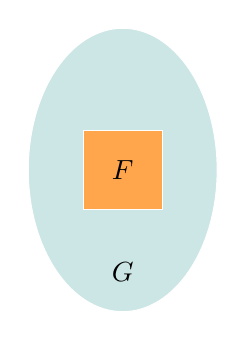
\begin{tikzpicture}
            \filldraw[fill=blue!50!green!20, draw=white] (0, 0) ellipse (1.2 and 1.8);
            \filldraw[fill=orange!70, draw=white] (-0.5, -0.5) rectangle (0.5, 0.5);
            \node at (0, 0) {$F$};
            \node at (0, -1.3) {$G$};
        \end{tikzpicture}
        \hspace{20pt}
        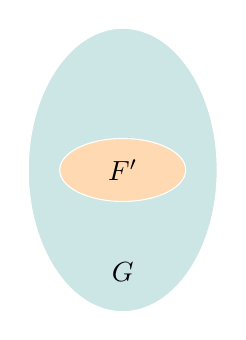
\begin{tikzpicture}
            \filldraw[fill=blue!50!green!20, draw=white] (0, 0) ellipse (1.2 and 1.8);
            \filldraw[fill=orange!30, draw=white] (0, 0) ellipse (0.8 and 0.4);
            \node at (0, 0) {$F'$};
            \node at (0, -1.3) {$G$};
        \end{tikzpicture}
        \hspace{20pt}
        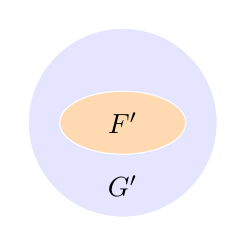
\begin{tikzpicture}
            \filldraw[fill=blue!10, draw=white] (0, 0) circle (1.2);
            \filldraw[fill=orange!30, draw=white] (0, 0) ellipse (0.8 and 0.4);
            \node at (0, 0) {$F'$};
            \node at (0, -0.8) {$G'$};
        \end{tikzpicture}
    \]


    或者我们可以先使用\hask{beta}来重新打包外部容器,然后应用\hask{fmap alpha}来重新打包所有内部容器。最终结果是相同的。

    \[
        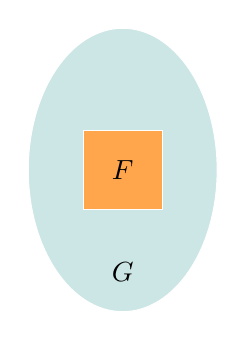
\begin{tikzpicture}
            \filldraw[fill=blue!50!green!20, draw=white] (0, 0) ellipse (1.2 and 1.8);
            \filldraw[fill=orange!70, draw=white] (-0.5, -0.5) rectangle (0.5, 0.5);
            \node at (0, 0) {$F$};
            \node at (0, -1.3) {$G$};
        \end{tikzpicture}
        \hspace{20pt}
        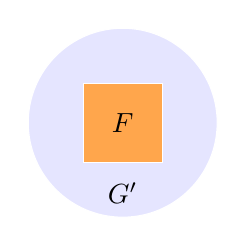
\begin{tikzpicture}
            \filldraw[fill=blue!10, draw=white] (0, 0) circle (1.2);
            \filldraw[fill=orange!70, draw=white] (-0.5, -0.5) rectangle (0.5, 0.5);
            \node at (0, 0) {$F$};
            \node at (0, -0.9) {$G'$};
        \end{tikzpicture}
        \hspace{20pt}
        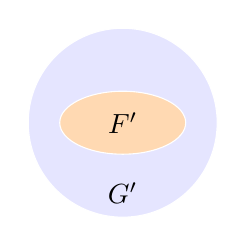
\begin{tikzpicture}
            \filldraw[fill=blue!10, draw=white] (0, 0) circle (1.2);
            \filldraw[fill=orange!30, draw=white] (0, 0) ellipse (0.8 and 0.4);
            \node at (0, 0) {$F'$};
            \node at (0, -0.9) {$G'$};
        \end{tikzpicture}
    \]


    \begin{exercise}
        实现\hask{safeHead}和\hask{reverse}的水平组合的两个版本。比较它们在各种参数上的作用。
    \end{exercise}

    \begin{exercise}
        同样做\hask{reverse}和\hask{safeHead}的水平组合。
    \end{exercise}

    \subsection{Whiskering}

    水平组合经常在其中一个自然变换是恒等变换时使用。这种组合有一个简写表示法。例如,$\alpha \circ id_F$写作$\alpha \circ F$。

    由于图的特征形状,这种组合被称为“Whiskering”。
    \[
        \begin{tikzcd}[column sep=huge]
            \mathcal{C}
            \arrow[r, "F"]
            &
            \mathcal{D}
            \arrow[bend left=50]{r}[name=U1, label=above:$G$]{}
            \arrow[bend right=50]{r}[name=D1, label=below:$G'$]{}
            &
            \mathcal{E}
            \arrow[shorten <=10pt,shorten >=10pt,Rightarrow,to path={(U1) -- node[label=left:$\alpha$] {} (D1)}]{}
        \end{tikzcd}
    \]
    在分量中,我们有:
    \[ (\alpha \circ F)_x = \alpha_{F x} \]

    让我们考虑如何将其翻译为Haskell。自然变换是一个多态函数。由于参数性,它对所有类型都是由同一个公式定义的。因此在右边Whiskering不会改变公式,它改变了函数签名。

    例如,如果这是\hask{alpha}的声明:
    \begin{haskell}
        alpha :: forall x. G x -> G' x
    \end{haskell}
    那么它的Whiskering版本将是:
    \begin{haskell}
        alpha_f :: forall x. G (F x) -> G' (F x)
        alpha_f = alpha
    \end{haskell}
    由于Haskell的类型推导,这种转换是隐式的。当调用一个多态函数时,我们不必指定执行自然变换的哪个分量——类型检查器会通过查看参数的类型来判断。

    此时的直觉是我们重新打包外部容器而保留内部容器不变。

    类似地,$id_H \circ \alpha$写作$H \circ \alpha$。
    \[
        \begin{tikzcd}[column sep=huge]
            \mathcal{D}
            \arrow[bend left=50]{r}[name=U, label=above:$G$]{}
            \arrow[bend right=50]{r}[name=D, label=below:$G'$]{}
            &
            \mathcal{E}
            \arrow[r, "H"]
            &
            \mathcal{F}
            \arrow[shorten <=10pt,shorten >=10pt,Rightarrow,to path={(U) -- node[label=left:$\alpha$] {} (D)}]{}
        \end{tikzcd}
    \]
    在分量中:
    \[(H \circ \alpha)_x = H (\alpha_x) \]

    在Haskell中,通过$H$提升$\alpha_x$是用\hask{fmap}完成的,因此给定:
    \begin{haskell}
        alpha :: forall x. G x -> G' x
    \end{haskell}
    Whiskering版本将是:
    \begin{haskell}
        h_alpha :: forall x. H (G x) -> H (G' x)
        h_alpha = fmap alpha
    \end{haskell}
    同样,Haskell的类型推导引擎会判断使用哪个版本的\hask{fmap}(在这里,它是\hask{Functor}实例\hask{G}的那个)。

    直觉上,这表明我们重新打包了内部容器的内容,同时保留外部容器不变。

    最后,在许多应用中,自然变换在两侧都进行了Whiskering:
    \[
        \begin{tikzcd}[column sep=huge]
            \mathcal{C}
            \arrow[r, "F"]
            &
            \mathcal{D}
            \arrow[bend left=50]{r}[name=U1, label=above:$G$]{}
            \arrow[bend right=50]{r}[name=D1, label=below:$G'$]{}
            &
            \mathcal{E}
            \arrow[shorten <=10pt,shorten >=10pt,Rightarrow,to path={(U1) -- node[label=left:$\alpha$] {} (D1)}]{}
            \arrow[r, "H"]
            &
            \mathcal{F}
        \end{tikzcd}
    \]
    在分量中,我们有:
    \[ (H \circ \alpha \circ F) x = H (\alpha_{F x})\]
    在Haskell中:
    \begin{haskell}
        h_alpha_f :: forall x. H (G (F x)) -> H (G' (F x))
        h_alpha_f = fmap alpha
    \end{haskell}

    这里的直觉是我们有一个三层容器;我们正在重新排列中间层,同时保留外层容器和所有内层容器不变。

    \subsection{交换律 (Interchange Law)}

    我们可以将垂直组合与水平组合结合起来,如下图所示:
    \[
        \begin{tikzcd}[column sep=huge]
            \mathcal{C}
            \arrow[bend left=60]{rr}[name=U, label=above:$F$]{}
            \arrow[]{rr}[name=M, label={[xshift=15pt, yshift=-5pt]:$G$}]{}
            \arrow[bend right=60]{rr}[name=D, label=below:$H$]{}
            &&
            \mathcal{D}
            \arrow[bend left=60]{rr}[name=U1, label=above:$F'$]{}
            \arrow[]{rr}[name=M1, label={[xshift=15pt, yshift=-5pt]:$G'$}]{}
            \arrow[bend right=60]{rr}[name=D1, label=below:$H'$]{}
            &&
            \mathcal{E}
            \arrow[shorten <=8pt, shorten >=8pt,Rightarrow, to path={(U) -- node[label=left:$\alpha$] {} (M)}]{}
            \arrow[shorten <=8pt, shorten >=8pt,Rightarrow, to path={(M) -- node[label=left:$\beta$] {} (D)}]{}
            \arrow[shorten <=8pt, shorten >=8pt,Rightarrow, to path={(U1) -- node[label=left:$\alpha'$] {} (M1)}]{}
            \arrow[shorten <=8pt, shorten >=8pt,Rightarrow, to path={(M1) -- node[label=left:$\beta'$] {} (D1)}]{}
        \end{tikzcd}
    \]
    交换律(Interchange law)规定组合的顺序并不重要:我们可以先做垂直组合,然后是水平组合;或者先做水平组合,然后是垂直组合。

\end{document}


\section{重访泛在构造 (Universal Constructions Revisited)}

老子说,最简单的模式是最清晰的。

我们已经看到了和、积、指数、自然数和列表的定义。

传统的定义这些数据类型的方法是探索它们的内部。这是集合论的方式:我们考察新集合的元素如何从旧集合的元素构造出来。一个和的元素要么是第一个集合的元素,要么是第二个集合的元素。一个积的元素是一对元素,依此类推。从工程的角度来看,我们是在观察对象。

在范畴论中,我们采取相反的方法。我们不关心对象的内部或它是如何实现的。我们关心的是对象的目的,它如何被使用,以及它如何与其他对象交互。我们从实用主义的角度看待对象。

这两种方法各有其优点。范畴论的方法出现较晚,因为你需要研究大量的实例才能看清楚模式。但一旦你看到了这些模式,你就会发现事物之间意想不到的联系,比如和与积之间的对偶性。

通过它们之间的联系来定义特定的对象需要考察它们可能与之交互的无限多个对象。

“告诉我你与宇宙的关系,我就会告诉你是谁。”

通过关于范畴中所有对象的映射来定义对象的过程被称为“泛在构造 (universal construction)”。

为什么自然变换 (natural transformations) 如此重要?这是因为大多数范畴构造涉及交换图 (commuting diagrams)。如果我们可以将这些图重构为自然性方块 (naturality squares),我们就能在抽象的阶梯上更进一步,并获得新的有价值的见解。

能够将大量的事实压缩成简洁优雅的公式,有助于我们发现新的模式。例如,我们会看到同态集之间的自然同构在范畴论中随处可见,最终引出了伴随 (adjunction) 的概念。

但首先,我们将详细研究几个例子,以了解范畴论简洁语言的含义。例如,我们将尝试解码这样的陈述:两个对象的和(或称余积)由以下自然同构定义:

\[
    [\mathbf{2}, \mathcal{C}](D, \Delta_x) \cong \mathcal{C}(a + b, x)
\]

\subsection{选择对象 (Picking objects)}

即使是指向一个对象这样简单的任务,在范畴论中也有特殊的解释。我们已经看到,指向一个集合的元素等同于从单元素集合中选择一个函数。同样,在范畴中选择一个对象等同于从单对象范畴中选择一个函子。或者,可以通过从另一个范畴中的常值函子 (constant functor) 来完成。

我们经常想要选择一对对象。这也可以通过从一个双对象的简图范畴中选择一个函子来完成。同样,选择一个箭头等同于从“行走箭头 (walking arrow)”范畴中选择一个函子,等等。

通过明智地选择我们的函子和它们之间的自然变换,我们可以重新表述到目前为止我们看到的所有泛在构造。

\subsection{作为自然变换的余脚 (Cospans as natural transformations)}

和的定义要求选择两个需要求和的对象;以及一个第三对象作为映射出去的目标。

\[
    \begin{tikzcd}
        a
        \arrow[dr, bend left, "\text{Left}"']
        \arrow[ddr, bend right, "f"']
        && b
        \arrow[dl, bend right, "\text{Right}"]
        \arrow[ddl, bend left, "g"]
        \\
        &a + b
        \arrow[d, dashed, "h"]
        \\
        & c
    \end{tikzcd}
\]

这个图可以进一步分解为两个更简单的形状,称为“余脚 (cospans)”:

\[
    \begin{tikzcd}
        a
        \arrow[dr, ""']
        && b
        \arrow[dl, ""]
        \\
        & x
    \end{tikzcd}
\]

要构造一个余脚,我们首先要选择一对对象。为此,我们从一个双对象范畴 $\mathbf{2}$ 开始。我们将其对象称为 $1$ 和 $2$。我们使用一个函子
\[ D \colon \mathbf{2} \to \mathcal{C} \]
来选择对象 $a$ 和 $b$:
\begin{align*}
    D\, 1 &= a \\
    D\, 2 &= b
\end{align*}
($D$ 代表“图 (diagram)”,因为这两个对象在 $\mathcal{C}$ 中形成了一个非常简单的由两个点组成的图。)

我们使用常值函子 (constant functor)
\[ \Delta_x \colon \mathbf{2} \to \mathcal{C} \]
来选择对象 $x$。这个函子将 $1$ 和 $2$ 都映射到 $x$(并将两个恒等箭头映射到 $id_x$)。

由于这两个函子都从 $\mathbf{2}$ 到 $\mathcal{C}$,我们可以在它们之间定义一个自然变换 $\alpha$。在这种情况下,它只是两个箭头的组合:
\begin{align*}
    \alpha_1 \colon D \, 1 \to \Delta_x 1 \\
    \alpha_2 \colon D \, 2 \to \Delta_x 2
\end{align*}
这些正是余脚中的两个箭头。

由于 $\mathbf{2}$ 中没有箭头(除了恒等箭头),所以 $\alpha$ 的自然性条件是显而易见的。

可能有许多余脚共享相同的三个对象——这意味着:在两个函子 $D$ 和 $\Delta_x$ 之间可能有许多自然变换。这些自然变换在函子范畴 $[\mathbf{2}, \mathcal{C}]$ 中形成了一个同态集,即:
\[ [\mathbf{2}, \mathcal{C}](D, \Delta_x) \]

\subsection{余脚的函子性 (Functoriality of cospans)}

让我们考虑当我们开始在余脚中改变对象 $x$ 时会发生什么。我们有一个映射 $F$,它将 $x$ 映射到 $x$ 上的余脚集合:
\[ F x = [\mathbf{2}, \mathcal{C}](D, \Delta_x) \]
这个映射在 $x$ 上表现为函子性。

要看到这一点,请考虑一个箭头 $m \colon x \to y$。这个箭头的提升是两个自然变换集合之间的映射:
\[ [\mathbf{2}, \mathcal{C}](D, \Delta_x) \to [\mathbf{2}, \mathcal{C}](D, \Delta_{y}) \]

这看起来可能非常抽象,直到你记住自然变换有分量,这些分量只是普通的箭头。左侧集合的一个元素是一个自然变换:
\[ \mu \colon D \to \Delta_x \]
它有两个对应于 $\mathbf{2}$ 中两个对象的分量。例如,我们有:
\[ \mu_1 \colon D \, 1 \to \Delta_x 1 \]
或者,使用 $D$ 和 $\Delta$ 的定义:
\[ \mu_1 \colon a \to x \]
这只是我们余脚的左腿。

同样,右侧集合的元素是一个自然变换:
\[ \nu \colon D \to \Delta_{y} \]
它在 $1$ 处的分量是一个箭头:
\[ \nu_1 \colon a \to y \]
我们可以通过将其与 $m \colon x \to y$ 后组合来从 $\mu_1$ 到 $\nu_1$。因此,$m$ 的提升是一个逐分量后组合 $(m \circ -)$:
\begin{align*}
    \nu_1 = m \circ \mu_1 \\
\end{align*}
\begin{align*}
    \nu_2 = m \circ \mu_2
\end{align*}

\subsection{和作为泛在余脚 (Sum as a universal cospan)}

在你可以在对 $a$ 和 $b$ 进行构造的所有余脚中,我们称为 $\text{Left}$ 和 $\text{Right}$ 的箭头在 $a + b$ 上汇聚的那个是非常特殊的。有一个唯一的映射从它映射到任何其他余脚——一个使两个三角形交换的映射。
\[
    \begin{tikzcd}
        a
        \arrow[dr, bend left, "\text{Left}"']
        \arrow[ddr, bend right, "f"']
        && b
        \arrow[dl, bend right, "\text{Right}"]
        \arrow[ddl, bend left, "g"]
        \\
        &a + b
        \arrow[d, dashed, "h"]
        \\
        & x
    \end{tikzcd}
\]

我们现在能够将这种条件转换为关于自然变换和同态集的陈述。箭头 $h$ 是同态集 $\mathcal{C}(a + b, x)$ 的元素。

$x$ 上的余脚是一个自然变换,即函子范畴中的同态集的元素:
\[ [\mathbf{2}, \mathcal{C}](D, \Delta_x) \]

这两个同态集都在各自的范畴中。而且它们都是集合,即 $\mathbf{Set}$ 范畴中的对象。这个范畴形成了函子范畴 $[\mathbf{2}, \mathcal{C}]$ 和“常规”范畴 $\mathcal{C}$ 之间的桥梁,尽管从概念上讲,它们似乎处于非常不同的抽象层次。

借用西格蒙德·弗洛伊德的话:“有时一个集合只是一个集合。”

我们的泛在构造是集合之间的双射或同构:
\[ [\mathbf{2}, \mathcal{C}](D, \Delta_x)  \cong \mathcal{C}(a + b, x) \]

此外,如果我们改变对象 $x$,这两边表现得像是从 $\mathcal{C}$ 到 $\mathbf{Set}$ 的函子。因此,问这个函子映射是否是自然同构是有意义的。

实际上,可以证明这个同构的自然性条件转化为和定义中的三角形的交换条件。因此,可以用一个方程来替代和的定义。

\subsection{积作为泛在跨度 (Product as a universal span)}

关于积的泛在构造,也可以做类似的论证。同样,我们从简图范畴 $\mathbf{2}$ 和函子 $D$ 开始。但这次我们使用一个相反方向的自然变换
\[ \alpha \colon \Delta_x \to D \]
这样的自然变换是一对箭头,形成一个“跨度 (span)”:
\[
    \begin{tikzcd}
        &x
        \arrow[dl, "f"']
        \arrow[dr, "g"]
        \\
        a
        && b
    \end{tikzcd}
\]
这些自然变换集合形成了函子范畴中的一个同态集:
\[[\mathbf{2}, \mathcal{C}](\Delta_x, D) \]

这个同态集的每个元素都与映射到积 $a \times b$ 的唯一映射 $h$ 一一对应。这样的映射是同态集 $\mathcal{C}(x, a \times b)$ 的成员。这种对应关系表示为同构:
\[ [\mathbf{2}, \mathcal{C}](\Delta_x, D)  \cong \mathcal{C}(x, a \times b) \]
可以证明,这个同构的自然性保证了此图中的三角形交换:
\[
    \begin{tikzcd}
        & x
        \arrow[d, dashed, "h"]
        \arrow[ddl, bend right, "f = \alpha_1"']
        \arrow[ddr, bend left, "g = \alpha_2"]
        \\
        &a \times b
        \arrow[dl, "\text{fst}"]
        \arrow[dr, "\text{snd}"']
        \\
        a = D\, 1 && b = D \, 2
    \end{tikzcd}
\]

\subsection{指数 (Exponentials)}

指数或函数对象由以下交换图定义:
\[
    \begin{tikzcd}
        x \times a
        \arrow[d, dashed, "h \times id_a"']
        \arrow[rd, "f"]
        \\
        b^a \times a
        \arrow[r, "\varepsilon_{a b}"']
        & b
    \end{tikzcd}
\]
这里,$f$ 是同态集 $\mathcal{C}(x \times a, b)$ 的一个元素,而 $h$ 是 $\mathcal{C}(x, b^a)$ 的一个元素。

这些集合之间的自然同构定义了指数对象。
\[\mathcal{C}(x \times a, b) \cong \mathcal{C}(x, b^a)\]

上述图中的 $f$ 是左侧的一个元素,而 $h$ 是右侧的相应元素。自然变换 $\alpha_x$(它还取决于 $a$ 和 $b$)将 $f$ 映射为 $h$。
\[ \alpha_x \colon \mathcal{C}(x \times a, b) \to \mathcal{C}(x, b^a) \]
在 Haskell 中,我们称其为 \hask{curry}。它的逆变换 $\alpha^{-1}$ 被称为 \hask{uncurry}。

与前面的例子不同,这里两个同态集都在同一个范畴中,因此很容易更详细地分析这个同构。特别是,我们希望看看交换条件:
\[  f = \varepsilon_{a b} \circ (h \times id_a) \]
如何从自然性中得出。

标准的 Yoneda 技巧是为 $x$ 进行替换,将其中一个同态集简化为一个自同态集,即源与目标相同的同态集。这将使我们能够选择该同态集的规范元素,即恒等箭头。

在我们的例子中,将 $b^a$ 替换为 $x$ 将允许我们选择 $h = id_{(b^a)}$。
\[
    \begin{tikzcd}
        b^a \times a
        \arrow[d, dashed, "id_{(b^a)} \times id_a"']
        \arrow[rd, "f"]
        \\
        b^a \times a
        \arrow[r, "\varepsilon_{a b}"']
        & b
    \end{tikzcd}
\]
这种情况下的交换条件告诉我们 $f = \varepsilon_{a b}$。换句话说,我们得到了关于 $\alpha$ 的 $\varepsilon_{a b}$ 的公式:
\[ \varepsilon_{a b} = \alpha_{x}^{-1} (id_{x}) \]
其中,$x$ 等于 $b^a$。

由于我们识别 $\alpha^{-1}$ 为 \hask{uncurry},识别 $\varepsilon$ 为函数应用,因此我们可以在 Haskell 中将其写为:
\begin{haskell}
    apply :: (a -> b, a) -> b
    apply = uncurry id
\end{haskell}
这最初可能令人惊讶,直到你意识到 \hask{(a->b,a)->b} 的柯里化导致 \hask{(a->b)->(a->b)}。

我们还可以将主同构的两边编码为 Haskell 函子:
\begin{haskell}
    data LeftFunctor  a b x = LF ((x, a) -> b)
\end{haskell}
\begin{haskell}
    data RightFunctor a b x = RF (x -> (a -> b))
\end{haskell}
它们都是在类型变量 \hask{x} 中的逆变函子。
\begin{haskell}
    instance Contravariant (LeftFunctor a b) where
    contramap g (LF f) = LF (f . bimap g id)
\end{haskell}
这表示 $g \colon x \to y$ 的提升由以下后组合给出:
\[ \mathcal{C}(y \times a, b) \xrightarrow{(- \circ (g \times id_a)) }  \mathcal{C}(x \times a, b)\]

类似地:
\begin{haskell}
    instance Contravariant (RightFunctor a b) where
    contramap g (RF h) = RF (h . g)
\end{haskell}
翻译为:
\[  \mathcal{C}(y, b^a) \xrightarrow{ (- \circ g) } \mathcal{C}(x, b^a) \]

自然变换 $\alpha$ 只是 \hask{curry} 的一个薄封装;它的逆变换是 \hask{uncurry}:

\begin{haskell}
    alpha :: forall a b x. LeftFunctor a b x -> RightFunctor a b x
    alpha (LF f) = RF (curry f)
\end{haskell}

\begin{haskell}
    alpha_1 :: forall a b x. RightFunctor a b x -> LeftFunctor a b x
    alpha_1 (RF h) = LF (uncurry h)
\end{haskell}

使用 $g \colon x \to y$ 的两种提升公式,以下是自然性方块:

\[
    \begin{tikzcd}
        \mathcal{C}(y \times a, b)
        \arrow[rr, "(- \circ (g \times id_a))"]
        \arrow[d, "\alpha_y"]
        & &
        \mathcal{C}(x \times a, b)
        \arrow[d, "\alpha_x"]
        \\
        \mathcal{C}(y, b^a)
        \arrow[rr, "(- \circ g)"]
        & &
        \mathcal{C}(x, b^a)
    \end{tikzcd}
\]

现在让我们将 Yoneda 技巧应用于它,并将 $y$ 替换为 $b^a$。这也使我们能够将 $g$(现在它从 $x$ 到 $b^a$)替换为 $h$。

\[
    \begin{tikzcd}
        \mathcal{C}(b^a \times a, b)
        \arrow[rr, "(- \circ (h \times id_a))"]
        \arrow[d, "\alpha_{(b^a)}"]
        & &
        \mathcal{C}(x \times a, b)
        \arrow[d, "\alpha_x"]
        \\
        \mathcal{C}(b^a, b^a)
        \arrow[rr, "(- \circ h)"]
        & &
        \mathcal{C}(x, b^a)
    \end{tikzcd}
\]

我们知道同态集 $\mathcal{C}(b^a, b^a)$ 至少包含恒等箭头,因此我们可以选择左下角的元素 $id_{(b^a)}$。

反转左侧的箭头,我们知道 $\alpha^{-1}$ 作用于恒等箭头会在左上角产生 $\varepsilon_{a b}$(这是 \hask{uncurry id} 技巧)。

$h$ 作用于恒等箭头的前置组合会在右下角产生 $h$。

$\alpha^{-1}$ 作用于 $h$ 会在右上角产生 $f$。

\[
    \begin{tikzcd}[
        every arrow/.style={draw,mapsto}
    ]
        \varepsilon_{a b}
        \arrow[rr, "(- \circ (h \times id_a))"]
        & &
        f
        \\
        id_{(b^a)}
        \arrow[u, "\alpha^{-1}"]
        \arrow[rr, "(- \circ h)"]
        & &
        h
        \arrow[u, "\alpha^{-1}"']
    \end{tikzcd}
\]
($\mapsto$ 箭头表示函数作用于集合元素的操作。)

因此,选择左下角的 $id_{(b^a)}$ 固定了其他三个角。特别是,我们可以看到,应用于 $\varepsilon_{a b}$ 的上箭头产生 $f$,这正是我们设定要推导的交换条件:
\[ \varepsilon_{a b} \circ (h \times id_a) = f \]


\section{Limits and Colimits}

In the previous section we defined the sum and the product using natural transformations. These were transformations between diagrams defined as functors from a very simple stick-figure category $\mathbf{2}$, one of the functors being the constant functor. 

Nothing prevents us from replacing the category $\mathbf{2}$ with something more complex. For instance, we could try categories that have non-trivial arrows between objects, or categories with infinitely many objects. 

There is a whole vocabulary built around such constructions. 

We used objects in the category $\mathbf{2}$ for indexing objects in the category $\mathcal{C}$. We can replace $\mathbf{2}$ with an arbitrary indexing category $\cat J$. A diagram in $\mathcal{C}$ is still defined as a functor $D \colon \cat J \to \mathcal{C}$. It picks objects in $\mathcal{C}$, but it also picks arrows between them.

As the second functor we'll still use the constant functor $\Delta_x \colon \cat J \to \mathcal{C}$.

A  natural transformation, that is an element of the hom-set
\[ [\cat J, \mathcal{C}](\Delta_x, D)  \]
is now called a \emph{cone}. Its dual, an element of
\[ [\cat J, \mathcal{C}](D, \Delta_x)  \]
is called a \emph{cocone}. They generalize the span and the cospan, respectively.

Diagramatically, cones and cocones look like this:
\[
 \begin{tikzcd}
  & x
\arrow[ddr, "g"]
 \arrow[ddl, "f"']
 \arrow[ddd, "h"]
 \\
\\
D 1 
\arrow[rr, red]
\arrow[rd, red]
&& D 2
\arrow[dl, red]
\\
& D 3
 \end{tikzcd}
 \qquad
\begin{tikzcd}
 D 1
 \arrow[rr, red]
 \arrow[dr, red]
 \arrow[dddr, "f"']
 && D 2
\arrow[dl, red]
 \arrow[dddl, "g"]
 \\
 & D 3
 \arrow[dd, "h"]
 \\
 \\
 & x
 \end{tikzcd}
 \]

Since the indexing category may now contain arrows, the naturality conditions for these diagrams are no longer trivial. The constant functor $\Delta_x$ shrinks all vertices to one, so naturality squares shrink to triangles. Naturality means that all triangles with $x$ in their apex must now commute. 

The universal cone, if it exists, is called the \emph{limit} of the diagram $D$, and is written as $\text{Lim}D$. Universality means that it satisfies the following isomorphism, natural in $x$:
\[ [\cat J, \mathcal{C}](\Delta_x, D)  \cong \mathcal{C}(x, \text{Lim}D) \]
For each cone with the apex $x$ there is a unique mapping from $x$ into the limit $ \text{Lim}D$.

A limit of a $\Set$-valued functor has a particularly simple characterization. It's a set of cones with the singleton set at the apex. Indeed, elements of the limit, that is functions from the singleton set to it, are in one-to-one correspondence with such cones:
\[ [\cat J, \mathcal{C}](\Delta_1, D)  \cong \mathcal{C}(1, \text{Lim}D) \]


Dually, the universal cocone is called a \emph{colimit}, and is described by the following natural isomorphism:
\[ [\cat J, \mathcal{C}](D, \Delta_x)  \cong \mathcal{C}( \text{Colim}D, x) \]


We can now say that a product is a limit (and a sum, a colimit) of a diagram from the indexing category $\mathbf{2}$.

Limits and colimits distill the essence of a pattern. 

A limit, like a product, is defined by its mapping-in property. A colimit, like a sum, is defined by its mapping-out property.

There are many interesting limits and colimits, and we'll see some when we discuss algebras and coalgebras.

\begin{exercise}
Show that the limit of a \index{walking arrow, limit}``walking arrow'' category, that is a two-object category with an arrow connecting the two objects, has the same elements as the first object in the diagram (``elements'' are the arrows from the terminal object).
\end{exercise}

\subsection{Equalizers}

A lot of high-school math involves learning how to solve equations or systems of equations. An equation equates the outcomes of two different ways of producing something. If we are allowed to subtract things, we usually shove everything to one side and simplify the problem to the one of calculating the zeros of some expression. In geometry, the same idea is expressed as the intersection of two geometric objects.

In category theory all these patterns are embodied in a single construction called an equalizer. An equalizer is a limit of a diagram whose pattern is given by a stick-figure category with two parallel arrows:
\[
\begin{tikzcd}
i \arrow[r, shift left=0.75ex]
  \arrow[r, shift right=0.75ex]
&
j
\end{tikzcd}
\]
The two arrows represent two ways of producing something. 

A functor from this category picks a pair of objects and a pair of morphisms in the target category. The limit of this diagram embodies an intersection of the two outcomes. It is an object $e$ with two arrows $p \colon e \to a$ and $p' \colon e \to b$.
\[
\begin{tikzcd}
& e
\arrow[dl, "p"']
\arrow[dr, gray, "p'"]
\\
a 
\arrow[rr, red, shift left=.75ex, "f"]
\arrow[rr, red, shift right=.75ex, "g"']
&&
b
\end{tikzcd}
\]
We have two commuting conditions:
\begin{align*}
p' &= f \circ h \\
p' &= g \circ h
\end{align*}
It means that $p'$ is fully determined by one of the equations, while the other turns into the constraints:
\[ f \circ p = g \circ p \]
Since the equalizer is the limit, it is the universal such pair, as illustrated in this diagram:
\[
\begin{tikzcd}
x
\arrow[d, dashed, "h"']
\arrow[dr, ""]
\\
e
\arrow[r, "p"']
&
a \arrow[r, red, shift left=0.75ex, "f"]
  \arrow[r, red, shift right=0.75ex, "g"']
&
b
\end{tikzcd}
\]

To develop the intuition for equalizers it's instructive to consider how it works for sets. As usual, the trick is to replace $x$ with the singleton set $1$:
\[
\begin{tikzcd}
1
\arrow[d, dashed, "e"']
\arrow[dr, "a"]
\\
E
\arrow[r, "p"']
&
A \arrow[r, red, shift left=0.75ex, "f"]
  \arrow[r, red, shift right=0.75ex, "g"']
&
B
\end{tikzcd}
\]
In this case $a$ is an element of $A$ such that $f a = g a$. That's just a way of saying that $a$ is the solution of a pair of equations. Universality means that there is a unique element $e$ of $E$ such that $p \circ e = a$. In other words, elements of $E$ are in one-to-one correspondence with the solutions of the system of equations. 

\subsection{Coequalizers}

What's dual to the idea of equating or intersecting? It's the process of discovering commonalities and organizing things into buckets. For instance, we can distribute integers into even and odd buckets. In category theory, this process of bucketizing is described by coequalizers.

A coequalizer is the colimit of the same diagram that we used to define the equalizer:
\[
\begin{tikzcd}
a 
\arrow[rr, red, shift left=.75ex, "f"]
\arrow[rr, red, shift right=.75ex, "g"']
\arrow[rd, gray, "q'"']
&&
b
\arrow[ld, "q"]
\\
& c
\end{tikzcd}
\]
This time, the arrow $q'$ is fully determined by $q$; and $q$ must satisfy the equation:
\[ q \circ f = q \circ g \]

Again, we can gain some intuition by considering a coequalizer of two functions acting on sets. 
\[
\begin{tikzcd}
A
\arrow[r, red, shift left=.75ex, "f"]
\arrow[r, red, shift right=.75ex, "g"']
&
B
\arrow[r, "q"]
& C
\end{tikzcd}
\]
An $x \in A$ is mapped to two elements $f x$ and $g x$ in $B$, but then $q$ maps them back to a single element of $C$. This element represents the bucket. Universality means that $C$ is a copy of $B$ in which the elements that were produced from the same $x$ have been identified.

Consider an example where $A$ is a set of pairs of integers \hask{(m, n)}, such that either both are even or both are odd.  We want to coequalize two functions that are the two projections \hask{(fst, snd)}. The equalizer set $C$ will have two elements corresponding to two buckets. We'll represent it as \hask{Bool}. The equalizing function \hask{q} selects the bucket:
\begin{haskell}
q :: Int -> Bool
q n = n `mod` 2 == 0 
\end{haskell}
Any function \hask{q'} that cannot distinguish between the components of our pairs can be uniquely factorized through the function \hask{h}:
\begin{haskell}
h :: (Int -> a) -> Bool -> a
h q' True  = g' 0
h q' False = g' 1
\end{haskell}

\begin{exercise}
Run a few tests that show that, in the example above, the factorization \hask{(h g') . q} gives the same result as \hask{g'} given by the following definition:
\begin{haskell}
import Data.Bits

q' :: Int -> Bool
q' x = testBit x 0
\end{haskell}

\end{exercise}
\begin{exercise}
What is the coequalizer of the pair \hask{(id, reverse)}, both of the type \hask{String->String}? Test its universality by factorizing the following function:
\begin{haskell}
q' :: String -> Maybe Char
q' s = if even len
       then Nothing
       else Just (s !! (len `div` 2))
  where len = length s
\end{haskell}
\end{exercise}

\subsection{The existence of the terminal object}

Lao Tzu says: great acts are made up of small deeds.

So far we've been studying limits of tiny diagrams, that is functors from simple stick-figure categories. Nothing, however, prevents us from defining limits and colimits where the patterns are taken to be infinite categories. But there is a gradation of infinities. When the objects in a category form a proper set, we call such a category  \index{small category}\emph{small}. Unfortunately, the very basic example, the category $\Set$ of sets, is not small. We know that there is no set of all sets. $\Set$ is a \index{large category}\emph{large} category. But at least all the hom-sets in $\Set$ are sets. We say that $\Set$ is \index{locally small category}\emph{locally small}. In what follows we'll be always working with locally small categories.

A small limit is a limit of a small diagram, that is a functor from a category whose objects and morphisms form sets. A category in which all small limits exist is called small complete, or just \emph{complete}. In particular, in such a category, a product of an arbitrary \emph{set} of objects exists. You can also equalize an arbitrary set of arrows between two objects. If such category is locally small, that means all equalizers exist.

Conversely, a (small) cocomplete category has all small colimits. In particular, such a category has all small coproducts and coequalizers.

The category $\Set$ is both complete and cocomplete. 


In a cocomplete locally small category there is a simple criterion for the existence of the terminal object: It's enough that a weakly terminal set exists. 

A \index{weakly terminal object}\emph{weakly terminal} object, just like the terminal object, has an arrow coming from any object; except that such an arrow is not necessarily unique. 

A \index{weakly terminal set}\emph{weakly terminal set} is a family of objects $t_i$ indexed by a set $I$ such that, for any object $c$ in $\cat C$ there exists an $i$ and an arrow $c \to t_i$. Such a set is also called a \index{solution set}\emph{solution set}.

\[
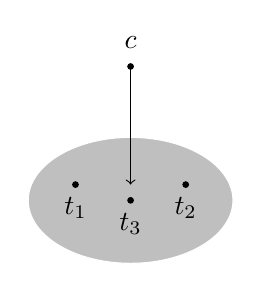
\begin{tikzpicture}
        \filldraw (0, 1.5) circle (1pt);
        \node at (0, 1.8) {$c$};
        
\filldraw[fill=gray!50, draw=white] (0, -0.2) ellipse (1.3 and 0.8);
        \filldraw (-0.7, 0) circle (1pt);
        \node at (-0.7, -0.3) {$t_1$};
        \filldraw (0.7, 0) circle (1pt);
        \node at (0.7, -0.3) {$t_2$};
        \filldraw (0, -0.2) circle (1pt);
        \node at (0, -0.5) {$t_3$};
        
    	\draw[->] (0, 1.5) -- (0, 0);
\end{tikzpicture}
\]

In a cocomplete category we can always construct a coproduct $\coprod_{i \in I} t_i$. This coproduct is a weakly terminal object, because there is an arrow to it from every $c$. This arrow is the composite of the arrow to some $t_i$ followed by the injection $\iota_i \colon t_i \to \coprod_{j \in I} t_j$.

Given a weakly terminal object, we can construct the (strongly) terminal object. We first define a subcategory $\cat T$ of $\cat C$ whose objects are $t_i$. Morphisms in $\cat T$ are all the morphisms in $\cat C$ that go between the objects of $\cat T$. This is called a \index{full subcategory}\emph{full} subcategory of $\cat C$. By our construction, $\cat T$ is small.

There is an obvious inclusion functor $F$ that embeds $\cat T$ in $\cat C$. This functor defines a small diagram in $\cat C$. It turns out that the colimit of this diagram is the terminal object in $\cat C$.

Dually, a similar construction can be used to define an initial object as a limit of a weakly initial set.

This property of solution sets will come handy in the proof of the Freyd's adjoint functor theorem.

\section{The Yoneda Lemma}

A functor from some category $\mathcal{C}$ to the category of sets can be thought of as a model of this category in $\mathbf{Set}$. Modeling, in general, is a lossy process: it discards some information. A constant $\Set$-valued functor is an extreme example: it maps the whole category to a single set and its identity function. 

A hom-functor produces a model of the category as viewed from a certain vantage point. The functor $\mathcal{C}(a, -)$, for instance, offers the panorama of $\mathcal{C}$ from the vantage point of $a$. It organizes all the arrows emanating from $a$ into neat packages that are connected by images of arrows that go between them, all in accordance with the original structure of the source category. 

\[
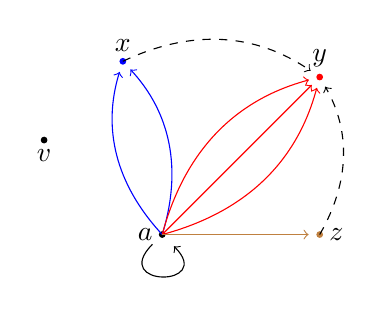
\begin{tikzpicture}
\def\ax{0}
\def\ay{0.5}
\def\xx{-0.5}
\def\xy{2.7}
\def\yx{2}
\def\yy{2.5}
\def\zx{2}
\def\zy{0.5}
\def\vx{-1.5}
\def\vy{1.7}
\filldraw[black] (\ax, \ay) circle (1 pt);
\node (a) at (\ax, \ay) {};
\node[left] at (\ax, \ay) {$a$};
\filldraw[blue] (\xx, \xy) circle (1 pt);
\node[above] at (\xx, \xy) {$x$};
\filldraw[red] (\yx, \yy) circle (1 pt);
\node[above] at (\yx, \yy) {$y$};
\filldraw[brown] (\zx, \zy) circle (1 pt);
\node[right] at (\zx, \zy) {$z$};
\filldraw[black] (\vx, \vy) circle (1 pt);
\node[below] at (\vx, \vy) {$v$};

\draw [->] (a) edge[out=225, in=315, loop] (a);

\draw[dashed] (\xx, \xy) edge[->, bend left, shorten > = 4 pt] (\yx, \yy);
\draw[dashed] (\zx, \zy) edge[->, bend right, shorten > = 4 pt] (\yx, \yy);

\draw[blue] (\ax, \ay) edge[->, bend left, shorten > = 4 pt] (\xx, \xy);
\draw[blue] (\ax, \ay) edge[->, bend right, shorten > = 4 pt] (\xx, \xy);

\draw[red] (\ax, \ay) edge[->, bend left, shorten > = 4 pt] (\yx, \yy);
\draw[red] (\ax, \ay) edge[->, bend right, shorten > = 4 pt] (\yx, \yy);
\draw[red] (\ax, \ay) edge[->, shorten > = 4 pt] (\yx, \yy);

\draw[brown] (\ax, \ay) edge[->, shorten > = 4 pt] (\zx, \zy);
\end{tikzpicture}
\hspace{80pt}
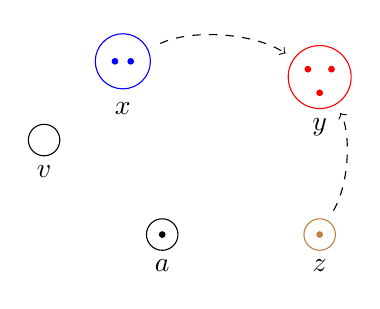
\begin{tikzpicture}
\def\ax{0}
\def\ay{0.5}
\def\xx{-0.5}
\def\xy{2.7}
\def\yx{2}
\def\yy{2.5}
\def\zx{2}
\def\zy{0.5}
\def\vx{-1.5}
\def\vy{1.7}
\def\sx{0.7}
\def\sy{1.6}

\node at (\sx, \sy) {$\Set$};

\draw[black] (\vx, \vy) circle (0.2);
\node[below] at (\vx, \vy - 0.2) {$v$};

\draw[black] (\ax, \ay) circle (0.2);
\filldraw[black] (\ax, \ay) circle (1 pt);
\node[below] at (\ax, \ay-0.2) {$a$};

\draw[blue] (\xx, \xy) circle (0.35);
\filldraw[blue] (\xx - 0.1, \xy) circle (1 pt);
\filldraw[blue] (\xx + 0.1, \xy) circle (1 pt);
\node[above] at (\xx, \xy - 0.8) {$x$};

\draw[red] (\yx, \yy) circle (0.4);
\filldraw[red] (\yx-0.15, \yy+0.1) circle (1 pt);
\filldraw[red] (\yx+0.15, \yy+0.1) circle (1 pt);
\filldraw[red] (\yx, \yy-0.2) circle (1 pt);
\node[below] at (\yx, \yy - 0.4) {$y$};

\draw[brown] (\zx, \zy) circle (0.2);
\filldraw[brown] (\zx, \zy) circle (1 pt);
\node[below] at (\zx, \zy - 0.2) {$z$};

\draw[dashed] (\xx, \xy) edge[->, bend left, shorten > = 15, shorten < = 15] (\yx, \yy);
\draw[dashed] (\zx, \zy) edge[->, bend right, shorten > = 15, shorten < = 10] (\yx, \yy);

\end{tikzpicture}
\]


Some vantage points are better than others. For instance, the view from the initial object is quite sparse. Every object $x$ is mapped to a singleton set $\cat C(0, x)$ corresponding to the unique mapping $0 \to x$. 

The view from the terminal object is more interesting: it maps all objects to their sets of (global) elements $\cat C(1, x)$. 

The Yoneda lemma may be considered one of the most profound statements, or one of the most trivial statements in category theory. Let's start with the profound version. 

Consider two models of $\mathcal{C}$ in $\mathbf{Set}$. The first one is given by the hom-functor  $\mathcal{C}(a, -)$. It's the panoramic, very detailed view of $\mathcal{C}$ from the vantage point of $a$. The second is given by some arbitrary functor $F \colon \mathcal{C} \to \mathbf{Set}$. Any natural transformation between them embeds one model in the other. It turns out that the set of all such natural transformations is fully determined by the set $F a$.

Since the set of natural transformation is the hom-set in the functor category $[\mathcal{C}, \mathbf{Set}]$, the formal statement of the Yoneda lemma takes the form:

\[ [\mathcal{C}, \mathbf{Set}]( \mathcal{C}(a, -), F) \cong F a \]
Moreover, this isomorphism is natural in both $a$ and $F$.

The reason this works is because all the mappings involved in this theorem are bound by the requirements of preserving the structure of the category $\mathcal{C}$ and the structure of its models. In particular, naturality conditions impose a huge set of constraints on the way the components of a natural transformation propagate from one point to another. 

The proof of the Yoneda lemma starts with a single identity arrow and lets naturality propagate it across the whole category.

Here's the sketch of the proof. It consists of two parts: First, given a natural transformation we construct an element of $F a$. Second, given an element of $F a$ we construct the corresponding natural transformation. 

First, let's pick an arbitrary element on the left-hand side of the Yoneda lemma: a natural transformation $\alpha$. Its component at $x$ is a function:
\[ \alpha_x \colon \mathcal{C}(a, x) \to F x \]
We can now apply the Yoneda trick: substitute $a$ for $x$:
\[ \alpha_a \colon \mathcal{C}(a, a) \to F a \]
and then pick the identity $id_a$ as the canonical element of $\mathcal{C}(a, a)$. The result is an element $\alpha_a (id_a)$ in the set $F a$. This defines a mapping in one direction, from natural transformations to elements of the set $F a$.

Now the other way around. Given an element $p$ of the set $F a$ we want to construct a natural transformation $\alpha$. First, we assign $p$ to be the action of $\alpha_a$ on $id_a \in \cat C(a, a)$. 

\[
\begin{tikzpicture}
\def\ax{0}
\def\ay{0.5}
\def\xx{-0.5}
\def\xy{3.7}
\filldraw[black] (\ax, \ay) circle (1 pt);
\node (a) at (\ax, \ay) {};
\node[left] at (\ax, \ay) {$a$};
\filldraw[blue] (\xx, \xy) circle (1 pt);
\node[above] at (\xx, \xy) {$x$};

\draw [->] (a) edge[out=225, in=315, loop] (a);
\node[right] at (\ax + 0.3, \ay - 0.35) {$id_a$};

\draw[blue] (\ax, \ay) edge[->, "$h$", bend right, shorten > = 4 pt] (\xx, \xy);

\end{tikzpicture}
\hspace{80pt}
\begin{tikzpicture}

\def\ax{0}
\def\ay{0.5}
\def\xx{-0.5}
\def\xy{3.7}

\def\fax{3}
\def\fay{0.5}
\def\fxx{3 - 0.5}
\def\fxy{3.7}

\def\px{\fax - 0.3}
\def\hx{\xx + 0.35}
% C(a,a)
\draw[black] (\ax, \ay) circle (0.2);
\filldraw[black] (\ax, \ay) circle (1 pt);
\node[below] at (\ax, \ay-0.2) {$\cat C (a, a)$};
% C(a,x)
\draw[black] (\xx, \xy) ellipse (0.7 and 0.4);

\filldraw[blue] (\xx + 0.35, \xy) circle (1 pt);
\node[left, blue] at (\hx, \xy) {$h$};

\node[above] at (\xx, \xy - 1.1) {$\cat C (a, x)$};
\draw[dashed] (\hx, \xy) edge[->, "$\alpha_x$", shorten > = 4 pt] (\fxx, \fxy);

% F a
\draw[red] (\fax, \fay) ellipse (0.7 and 0.4);
\filldraw[red] (\px, \fay) circle (1 pt);
\node[right, red] at (\px, \fay) {$p$};
\node[right, red] at (\fax + 0.7, \fay) {$F a$};
\draw[dashed] (\ax, \ay) edge[->, "$\alpha_a$", shorten > = 3 pt] (\px, \fay);
% F x
\draw[red] (\fxx, \fxy) circle (0.4);
\filldraw[red] (\fxx, \fxy) circle (1 pt);
\node[right, red] at (\fxx + 0.35, \fxy) {$F x$};

\draw[blue] (\px, \fay) edge[->, "$F h$", bend right, shorten > = 12, shorten < = 12] (\fxx, \fxy);

\end{tikzpicture}
\]


Now let's take an arbitrary object $x$ and an arbitrary element of $\cat C(a, x)$. The latter is an arrow $h \colon a \to x$. Our natural transformation must map it to an element of $F x$. We can do it by lifting the arrow $h$ using $F$. We get a function:
\[F h \colon F a \to F x \]
We can apply this function to $p$ and get an element of $F x$. We take this element to be the action of $\alpha_x$ on $h$:
\[ \alpha_x h = (F h) p \]

The isomorphism in the Yoneda lemma is natural both in $a$ and in $F$. The latter means that you can ``move'' from the functor $F$ to another functor $G$ by applying an arrow in the functor category, that is a natural transformation. This is quite a leap in the levels of abstraction, but all the definitions of functoriality and naturality work equally well in the functor category, where objects are functors, and arrows are natural transformations.

\begin{exercise}
Fill in the gap in the proof when $F a$ is empty.
\end{exercise}
\begin{exercise}
Show that the mapping 
\[ \mathcal{C}(a, x) \to F x\]
defined above is a natural transformation. Hint: Vary $x$ using some $f \colon x \to y$.
\end{exercise}
\begin{exercise}
Show that the formula for $\alpha_x$ can be derived from the assumption that $\alpha_a (id_a) = p$ and the naturality condition. Hint: The lifting of $h$ by the hom-functor $\cat C(a, h)$ is given by post-composition.
\end{exercise}

\subsection{Yoneda lemma in programming}

Now for the trivial part: The proof of the Yoneda lemma translates directly to Haskell code. We start with the type of natural transformation between the hom-functor \hask{a->x} and some functor \hask{f}, and show that it's equivalent to the type of \hask{f} acting on \hask{a}.
\begin{haskell}
forall x. (a -> x) -> f x.   -- is isomorphic to (f a)
\end{haskell}
We produce a value of the type \hask{(f a)} using the standard Yoneda trick
\begin{haskell}
yoneda :: Functor f => (forall x. (a -> x) -> f x) -> f a
yoneda g = g id
\end{haskell}
Here's the inverse mapping:
\begin{haskell}
yoneda_1 :: Functor f => f a -> (forall x. (a -> x) -> f x)
yoneda_1 y = \h -> fmap h y
\end{haskell}

Note that we are cheating a little by mixing types and sets. The Yoneda lemma in the present formulation works with  $\mathbf{Set}$-valued functors. Again, the correct incantation is to say that we use the enriched version of the Yoneda lemma in a self-enriched category.

The Yoneda lemma has some interesting applications in programming. For instance, let's consider what happens when we apply the Yoneda lemma to the identity functor. We get the isomorphism between the type \hask{a} (the identity functor acting on \hask{a}) and
\begin{haskell}
forall x. (a -> x) -> x
\end{haskell}
We interpret this as saying that any data type \hask{a} can be replaced by a higher order polymorphic function. This function takes another function---called a handler, a callback, or a \emph{continuation}---as an argument. 

This is the standard continuation passing transformation that's used a lot in distributed programming, for instance when the value of type \hask{a} has to be retrieved from a remote server. It's also useful as a program transformation that turns recursive algorithms into tail-recursive functions.

Continuation-passing style is difficult to work with because the composition of continuations is highly nontrivial, resulting in what programmers often call a ``callback hell.'' Fortunately continuations form a monad, which means their composition can be hidden behind the \hask{do} notation.

\subsection{The contravariant Yoneda lemma}

By reversing a few arrow, the Yoneda lemma can be applied to contravariant functors as well. It works on natural transformations between the contravariant hom-functor $\mathcal{C}(-, a)$ and a contravariant functor $F$:

\[ [\mathcal{C}^{op}, \mathbf{Set}]( \mathcal{C}(-, a), F) \cong F a \]

This is the Haskell implementation of the mapping:
\begin{haskell}
coyoneda :: Contravariant f => (forall x. (x -> a) -> f x) -> f a
coyoneda g = g id
\end{haskell}
And this is the inverse transformation:
\begin{haskell}
coyoneda_1 :: Contravariant f => f a -> (forall x. (x -> a) -> f x)
coyoneda_1 y = \h -> contramap h y
\end{haskell}

\section{Yoneda Embedding}

In a closed category, we have exponential objects that serve as stand-ins for hom-sets. This is obviously a thing in $\Set$, where hom-sets, being sets, are automatically objects in $\Set$. 

On the other hand, in the category of categories  $\mathbf{Cat}$, hom-sets are \emph{sets} of functors, and it's not immediately obvious that they can be promoted to objects in $\mathbf{Cat}$---that is, categories. But, as we've seen before, they can! Functors between any two categories form a functor \emph{category}.

Because of that, it's possible to curry functors just like we curried functions. A functor from a product category can be viewed as a functor returning a functor. In other words, $\mathbf{Cat}$ is a closed (symmetric) monoidal category.

In particular, we can apply currying to the hom-functor $\mathcal{C}(a, b)$. It is a profunctor, or a functor from the product category:
\[ \mathcal{C}^{op} \times \mathcal{C} \to  \mathbf{Set} \]
But it's also a contravariant functor in the first argument $a$. And for every $a$ in  $\mathcal{C}^{op}$  it produces a covariant functor $\mathcal{C}(a, -)$, which is an object in the functor category $ [\mathcal{C},  \mathbf{Set}] $. We can write this mapping as:
\[ \mathcal{C}^{op} \to [\mathcal{C},  \mathbf{Set}] \]
Alternatively, we can fix $b$ and produce a contravariant functor $\mathcal{C}(-, b)$. This mapping can be written as
\[ \mathcal{C} \to [\mathcal{C}^{op},  \mathbf{Set}] \]
Both mappings are functorial, which means that, for instance, an arrow in $\mathcal{C}$ is mapped to a natural transformation in $[\mathcal{C}^{op},  \mathbf{Set}]$.

These $\mathbf{Set}$-valued functor categories are common enough that they have special names. The functors in $[\mathcal{C}^{op},  \mathbf{Set}]$ are called \index{presheaves}\emph{presheaves}, and the ones in $[\mathcal{C},  \mathbf{Set}]$ are called \index{co-presheaves}\emph{co-presheaves}. (The names come from algebraic topology.)

Let's focus our attention on the following reading of the hom-functor:
\[ \mathcal{Y} \colon \mathcal{C} \to [\mathcal{C}^{op},  \mathbf{Set}] \]
It takes an object $x$ and maps it to a presheaf 
\[ \mathcal Y_x = \mathcal{C}(-, x) \]
which can be visualized as the totality of views of $x$ from all possible directions.

Let's also review its action on arrows. The functor $\mathcal{Y}$ lifts an arrow $f \colon x \to y$ to a mapping of presheaves:
\[ \alpha \colon \mathcal{C}(-, x) \to \mathcal{C}(-, y) \]
The component of this natural transformation at some $z$ is a function between hom-sets:
\[ \alpha_z \colon \mathcal{C}(z, x) \to \mathcal{C}(z, y) \]
which is simply implemented as the post-composition $(f \circ -)$.

Such a functor $\mathcal{Y}$ can be thought of as creating a model of $\mathcal{C}$ in the presheaf category. But this is no run-of-the-mill model---it's an \emph{embedding} of one category inside another. This particular one is called the \emph{Yoneda embedding} and the functor $\mathcal{Y}$ is called the \index{Yoneda functor}\emph{Yoneda functor}. 

First of all, every object of $\mathcal{C}$ is mapped to a \emph{different} object (presheaf) in $[\mathcal{C}^{op},  \mathbf{Set}]$. We say that it's \index{injection}\emph{injective on objects}. 

But that's not all: every arrow in $\mathcal{C}$ is mapped to a \emph{different} arrow. We say that the embedding functor is \index{faithful functor}\emph{faithful}. 

If that weren't enough, the mapping of hom-sets is also \index{surjection}\emph{surjective}, meaning that every arrow between objects in $[\mathcal{C}^{op},  \mathbf{Set}]$ comes from some arrow in $\mathcal{C}$. We say that the functor is \index{full functor}\emph{full}. 

Altogether, the embedding is \emph{fully faithful}, that is the mapping of arrows is one-to-one. However, in general, the Yoneda embedding is \emph{not} surjective on objects, hence the word ``embedding.''

The fact that the embedding is fully faithful is the direct consequence of the Yoneda lemma. Indeed, we know that, for any functor $F \colon \mathcal{C}^{op} \to \mathbf{Set}$, we have a natural isomorphism:
\[ [\mathcal{C}^{op}, \mathbf{Set}]( \mathcal{C}(-, x), F) \cong F x \]
In particular, we can substitute another hom-functor $\mathcal{C}(-, y)$ for $F$ to get:
\[ [\mathcal{C}^{op}, \mathbf{Set}]( \mathcal{C}(-, x), \mathcal{C}(-, y)) \cong \mathcal{C}(x, y)\]
The left-hand side is the hom-set in the presheaf category and the right-hand side is the hom-set in $\mathcal{C}$. They are isomorphic, which proves that the embedding is fully faithful. In fact, the Yoneda lemma tells us that the isomorphism is natural in $x$ and $y$. 

Let's have a closer look at this isomorphism. Let's pick an element of the right-hand set $\mathcal{C}(x, y)$--- an arrow $f \colon x \to y$. The isomorphism maps it to a natural transformation whose component at $z$ is a function:
\[ \mathcal{C}(z, x) \to \mathcal{C}(z, y) \]
This mapping is implemented as post-composition $(f \circ -)$.

In Haskell, we would write it as:
\begin{haskell}
toNatural :: (x -> y) -> (forall z. (z -> x) -> (z -> y))
toNatural f = \h -> f . h 
\end{haskell}
In fact, this syntax works too:
\begin{haskell}
toNatural f = (f . )
\end{haskell}
The inverse mapping is:
\begin{haskell}
fromNatural :: (forall z. (z -> x) -> (z -> y)) -> (x -> y)
fromNatural alpha = alpha id
\end{haskell}
(Notice the use of the Yoneda trick again.)

This isomorphism maps identity to identity and composition to composition. That's because it's implemented as post-composition, and post-composition preserves both identity and composition. We've shown this fact before, in the chapter on isomorphisms:
\[ ((f \circ g) \circ -) = (f \circ -) \circ (g \circ -) \]

Because it preserves composition and identity, this isomorphism also preserves \emph{isomorphisms}. So if $x$ is isomorphic to $y$ then the presheaves $ \mathcal{C}(-, x)$ and $ \mathcal{C}(-, y)$ are isomorphic, and vice versa. 

This is exactly the result that we've been using all along to prove numerous isomorphisms in previous chapters. If the hom-sets are naturally isomorphic, then the objects are isomorphic. 

The Yoneda embedding builds on the idea that there is nothing more to an object than its relationships with other objects. The presheaf $\cat C (-, a)$, like a hologram, encodes the totality of views of $a$ from the perspective of the whole category $\cat C$. The Yoneda embedding tells us that, when we combine all these individual holograms, we get a perfect hologram of the whole category.

\section{Representable Functors}

Objects in a  co-presheaf category are functors that assign sets to objects in $\mathcal{C}$. Some of these functors work by picking a reference object $a$ and assigning,  to all objects $x$, their hom-sets  $\mathcal{C}(a, x)$:
\[ F x = \cat C(a, x) \]
Such functors, and all the functors isomorphic to those, are called \emph{representable}. The whole functor is ``represented'' by a single object $a$. 

In a closed category, the functor which assigns  to every object $x$ the set of elements of the exponential object $x^a$ is represented by $a$. This is because the set of elements of $x^a$ is isomorphic to $\mathcal{C}(a, x)$:
\[\mathcal{C}(1, x^a) \cong \mathcal{C}(1 \times a, x) \cong \mathcal{C} (a, x)\]

Seen this way, the representing object $a$ is like a logarithm of a functor. 

The analogy goes deeper: just like a logarithm of a product is a sum of logarithms, a representing object for a product data type is a sum. For instance, the functor that squares its argument using a product, $F x = x \times x$, is represented by $2$, which is the sum $1 + 1$. Indeed, we've seen before that $x \times x \cong x^2$.

Representable functors play a very special role in the category of $ \mathbf{Set}$-valued functors. Notice that the Yoneda embedding maps all objects of $\mathcal{C}$ to representable presheaves. It maps an object $x$ to a presheaf represented by $x$: 

\[  \mathcal{Y} \colon x \mapsto \mathcal{C}(-, x) \]

We can find the entire category  $\mathcal{C}$, objects and morphisms, embedded inside the presheaf category as representable functors. The question is, what else is there in the presheaf category ``in between'' representable functors?

Just like rational numbers are dense among real numbers, so representables are ``dense'' among (co-) presheaves. Every real number may be approximated by rational numbers. Every presheaf is a colimit of representables (and every co-presheaf, a limit). We'll come back to this topic when we talk about (co-) ends.

\begin{exercise}
Describe limits and colimits as representing objects. What are the functors they represent?
\end{exercise}
\begin{exercise}
Consider a \emph{singleton functor} $F \colon \cat C \to \Set$ that assigns to each object $c$ a singleton set $\{c\}$ that contains just that object (that is, a different singleton for every object). Define the action of $F$ on arrows. Show that $F$ being representable is equivalent to $\cat C$ having an initial object.
\end{exercise}

\subsection{The guessing game}

The idea that objects can be described by the way they interact with other objects is sometimes illustrated by playing an imaginary guessing game. One category theorist picks a secret object in a category, and the other has to guess which object it is (up to isomorphism, of course). 

The guesser is allowed to point at objects, and use them as ``probes'' into the secret object. The opponent is supposed to respond each time with a set: the set of arrows from the probing object $a$ to the secret object $x$. This, of course, is the hom-set $\mathcal{C}(a, x)$. 

The totality of these answers, as long as the opponent is not cheating, will define a presheaf $F \colon \mathcal{C}^{op} \to \mathbf{Set}$, and the object they are hiding is its representing object. 

But how do we know that the second category theorist in not cheating? To test that, we ask questions about arrows. For every arrow we select, they should give us a function between two sets---the sets they gave us for its endpoints. We can then check if all identity arrows are mapped to identity functions, and whether compositions of arrows map to compositions of functions. In other words, we'll be able to verify that $F$ is indeed a functor. 

However, a clever enough opponent may still fool us. The presheaf they are revealing to us may describe a fantastic object---a figment of their imagination---and we won't be able to tell. It turns out that such fantastic beasts are often as interesting as the real ones. 

\subsection{Representable functors in programming}

In Haskell, we define a class of representable functors using two functions that witness the isomorphism: 
\[ F x = \cat C(a, x) \]
The first one, \hask{tabulate}, turns a function into a lookup table; and the second, \hask{index}, uses the representing type \hask{Key} to index into it.

\begin{haskell}
class Representable f where
  type Key f :: Type
  tabulate :: (Key f -> x) -> f x
  index    :: f x -> (Key f -> x)
\end{haskell}

Algebraic data types that use sums are not representable (there is no formula for taking a logarithm of a sum). For instance, the list type is defined as a sum, so it's not representable. However, an infinite stream is. 

Conceptually, a stream is like an infinite tuple, which is technically a product. Such a stream is represented by the type of natural numbers. In other words, an infinite stream is equivalent to a mapping out of natural numbers. 
\begin{haskell}
data Stream a = Stm a (Stream a)
\end{haskell}
Here's the instance definition:
\begin{haskell}
instance Representable Stream where
  type Key Stream = Nat
  tabulate g = tab Z
    where
      tab n = Stm (g n) (tab (S n))
  index stm = \n -> ind n stm
    where
      ind Z (Stm a _) = a
      ind (S n) (Stm _ as) = ind n as
\end{haskell}
Representable types are useful for implementing \index{memoization} memoization of functions.

\begin{exercise}
Implement the \hask{Representable} instance for \hask{Pair}:
\begin{haskell}
data Pair x = Pair x x
\end{haskell}
\end{exercise}

\begin{exercise}
Is the constant functor that maps everything to the terminal object representable? Hint: what's the logarithm of 1?

In Haskell, such a functor could be implemented as:
\begin{haskell}
data Unit a = U
\end{haskell}
Implement the instance of \hask{Representable} for it.
\end{exercise}

\begin{exercise}
The list functor is not representable. But can it be considered a sum or representables?
\end{exercise}

\section{2-category  $\mathbf{Cat}$ }

In the category of categories, $\mathbf{Cat}$, the hom-sets are not ``just'' sets. Each of them can be promoted to a functor category, with natural transformations playing the role of arrows. This kind of structure is called a 2-category. 

In the language of 2-categories, objects are called \index{0-cells}0-cells, arrows between them are called \index{1-cells}1-cells, and arrows between arrows are called \index{2-cells}2-cells. 

The obvious generalization of that picture would be to have 3-cells that go between 2-cells and so on. An \index{$n$-category}$n$-category has cells going up to the $n$-th level. 

But why not have arrows going all the way? Enter \index{infinity categories}infinity categories. Far from being a curiosity, $\infty$-categories have practical applications. For instance they are used in algebraic topology to describe points, paths between points, surfaces swiped by paths, volumes swiped by surfaces, and so on, ad infinitum. 

\section{Useful Formulas}
\begin{itemize}
\item Yoneda lemma for covariant functors:
\[ [\mathcal{C}, \mathbf{Set}]( \mathcal{C}(a, -), F) \cong F a \]
\item Yoneda lemma for contravariant functors:
\[ [\mathcal{C}^{op}, \mathbf{Set}]( \mathcal{C}(-, a), F) \cong F a \]
\item Corollaries to the Yoneda lemma:
\begin{align*}
 [\mathcal{C}, \mathbf{Set}]( \mathcal{C}(x, -), \mathcal{C}(y, -)) &\cong \mathcal{C}(y, x) \\
 [\mathcal{C}^{op}, \mathbf{Set}]( \mathcal{C}(-, x), \mathcal{C}(-, y)) &\cong \mathcal{C}(x, y)
\end{align*}

\end{itemize}

\end{document}